\documentclass[journal,12pt,twocolumn]{IEEEtran}

\usepackage{setspace}
\usepackage{gensymb}


\singlespacing

\usepackage[cmex10]{amsmath}
%\usepackage{amsthm}
%\interdisplaylinepenalty=2500
%\savesymbol{iint}
%\usepackage{txfonts}
%\restoresymbol{TXF}{iint}
%\usepackage{wasysym}
\usepackage{amsthm}

\usepackage{mathrsfs}
\usepackage{txfonts}
\usepackage{stfloats}
\usepackage{bm}
\usepackage{cite}
\usepackage{cases}
\usepackage{subfig}

\usepackage{longtable}
\usepackage{multirow}

\usepackage{enumitem}
\usepackage{mathtools}
\usepackage{steinmetz}
\usepackage{tikz}
\usepackage{circuitikz}
\usepackage{verbatim}
\usepackage{tfrupee}
\usepackage[breaklinks=true]{hyperref}

\usepackage{tkz-euclide} %loads TikZ and tkz-base

\usetikzlibrary{calc,math}
\usepackage{listings}
    \usepackage{color}                                          
    \usepackage{array}                                          
    \usepackage{longtable}                                      
    \usepackage{calc}                                           
    \usepackage{multirow}                                       
    \usepackage{hhline}                                         
    \usepackage{ifthen}
    \usepackage{lscape}     
\usepackage{multicol}
\usepackage{chngcntr}

\DeclareMathOperator*{\Res}{Res}

\renewcommand\thesection{\arabic{section}}
\renewcommand\thesubsection{\thesection.\arabic{subsection}}
\renewcommand\thesubsubsection{\thesubsection.\arabic{subsubsection}}

\renewcommand\thesectiondis{\arabic{section}}
\renewcommand\thesubsectiondis{\thesectiondis.\arabic{subsection}}
\renewcommand\thesubsubsectiondis{\thesubsectiondis.\arabic{subsubsection}}

\hyphenation{op-tical net-works semi-conduc-tor}
\def\inputGnumericTable{}                                 %%

\lstset{
%language=C,
frame=single, 
breaklines=true,
columns=fullflexible
}

\begin{document}

\newtheorem{theorem}{Theorem}[section]
\newtheorem{problem}{Problem}
\newtheorem{proposition}{Proposition}[section]
\newtheorem{lemma}{Lemma}[section]
\newtheorem{corollary}[theorem]{Corollary}
\newtheorem{example}{Example}[section]
\newtheorem{definition}[problem]{Definition}

\newcommand{\BEQA}{\begin{eqnarray}}
\newcommand{\EEQA}{\end{eqnarray}}
\newcommand{\define}{\stackrel{\triangle}{=}}

\bibliographystyle{IEEEtran}

\providecommand{\mbf}{\mathbf}
\providecommand{\pr}[1]{\ensuremath{\Pr\left(#1\right)}}
\providecommand{\qfunc}[1]{\ensuremath{Q\left(#1\right)}}
\providecommand{\sbrak}[1]{\ensuremath{{}\left[#1\right]}}
\providecommand{\lsbrak}[1]{\ensuremath{{}\left[#1\right.}}
\providecommand{\rsbrak}[1]{\ensuremath{{}\left.#1\right]}}
\providecommand{\brak}[1]{\ensuremath{\left(#1\right)}}
\providecommand{\lbrak}[1]{\ensuremath{\left(#1\right.}}
\providecommand{\rbrak}[1]{\ensuremath{\left.#1\right)}}
\providecommand{\cbrak}[1]{\ensuremath{\left\{#1\right\}}}
\providecommand{\lcbrak}[1]{\ensuremath{\left\{#1\right.}}
\providecommand{\rcbrak}[1]{\ensuremath{\left.#1\right\}}}
\theoremstyle{remark}
\newtheorem{rem}{Remark}
\newcommand{\sgn}{\mathop{\mathrm{sgn}}}
\providecommand{\abs}[1]{\left\vert#1\right\vert}
\providecommand{\res}[1]{\Res\displaylimits_{#1}} 
\providecommand{\norm}[1]{\left\lVert#1\right\rVert}
%\providecommand{\norm}[1]{\lVert#1\rVert}
\providecommand{\mtx}[1]{\mathbf{#1}}
\providecommand{\mean}[1]{E\left[ #1 \right]}
\providecommand{\fourier}{\overset{\mathcal{F}}{ \rightleftharpoons}}
%\providecommand{\hilbert}{\overset{\mathcal{H}}{ \rightleftharpoons}}
\providecommand{\system}{\overset{\mathcal{H}}{ \longleftrightarrow}}
	%\newcommand{\solution}[2]{\textbf{Solution:}{#1}}
\newcommand{\solution}{\noindent \textbf{Solution: }}
\newcommand{\cosec}{\,\text{cosec}\,}
\providecommand{\dec}[2]{\ensuremath{\overset{#1}{\underset{#2}{\gtrless}}}}
\newcommand{\myvec}[1]{\ensuremath{\begin{pmatrix}#1\end{pmatrix}}}
\newcommand{\mydet}[1]{\ensuremath{\begin{vmatrix}#1\end{vmatrix}}}

\numberwithin{equation}{subsection}

\makeatletter
\@addtoreset{figure}{problem}
\makeatother

\let\StandardTheFigure\thefigure
\let\vec\mathbf

\renewcommand{\thefigure}{\theproblem}

\def\putbox#1#2#3{\makebox[0in][l]{\makebox[#1][l]{}\raisebox{\baselineskip}[0in][0in]{\raisebox{#2}[0in][0in]{#3}}}}
     \def\rightbox#1{\makebox[0in][r]{#1}}
     \def\centbox#1{\makebox[0in]{#1}}
     \def\topbox#1{\raisebox{-\baselineskip}[0in][0in]{#1}}
     \def\midbox#1{\raisebox{-0.5\baselineskip}[0in][0in]{#1}}
\vspace{3cm}

\title{Assignment 2}
\author{Surbhi Agarwal}

\maketitle

\newpage

%\tableofcontents

\bigskip

\renewcommand{\thefigure}{\theenumi}
\renewcommand{\thetable}{\theenumi}

\begin{abstract}
This document finds the foot of the perpendicular from the origin to the given planes
\end{abstract}

Download all python codes from 
%
\begin{lstlisting}
https://github.com/surbhi0912/EE5609/tree/master/Assignment2/codes\end{lstlisting}
%
and latex-tikz codes from 
%
\begin{lstlisting}
https://github.com/surbhi0912/EE5609/tree/master/Assignment2
\end{lstlisting}
%
\section{Problem}
For the following planes, find the coordinates of the foot of the perpendicular drawn from the origin

a) $\myvec{2&3&4}\vec{x} = 12$

b) $\myvec{3&4&-6}\vec{x} = 0$

c) $\myvec{1&1&1}\vec{x} = 1$

d) $\myvec{0&5&0}\vec{x} = -8$
\section{Explanation}
The equation of a plane is given as
\begin{align}\label{e1}
    \vec{n}^T\vec{x} = c
\end{align}
where $\vec{n}$ = normal vector to the plane

Let $\vec{O} = \myvec{0\\0\\0}$ be the origin and $\vec{P} = \myvec{x_1\\y_1\\z_1}$ be the foot of the perpendicular drawn from the origin to the plane.

The position vector from $\vec{O}$ to $\vec{P}$ is $(\vec{P} - \vec{O})$

Since $(\vec{P} - \vec{O})$ is perpendicular to the plane, it is parallel to the normal of the plane $\vec{n}$. So,
\begin{align}
    \vec{P} - \vec{O} = k\vec{n}\\
    \vec{P} = k\vec{n} + \vec{O}
\end{align}
where $k$ is any scalar quantity.

Since $\vec{O}$ is a null vector,
\begin{align}\label{e2}
    \implies\vec{P} = k\vec{n}
\end{align}
Since $\vec{P}$ lies on the given plane, it must satisfy the equation of the plane. Therefore,
\begin{align}
    \vec{n}^T\vec{P} = c\\
    \implies\vec{n}^T(k\vec{n}) = c\\
    \label{e3}\implies k\vec{n}^T\vec{n} = c
\end{align}
\section{Solution}
a)$\myvec{2&3&4}\vec{x} = 12$

Comparing with \eqref{e1}, we get $\vec{n}^T = \myvec{2&3&4}$ and  $c=12$. Using this in \eqref{e3}
\begin{align}
	k\myvec{2&3&4}\myvec{2\\3\\4} = 12\\
	\implies 29k = 12\\
	\implies k = \frac{12}{29}
\end{align}
\begin{align}
	\vec{P} = k\vec{n}
	\implies\vec{P} = \frac{12}{29}\myvec{2\\3\\4}\\
	\implies\vec{P}= \myvec{\dfrac{24}{29}\\\dfrac{36}{29}\\\dfrac{48}{29}}
\end{align}
b)$\myvec{3&4&-6}\vec{x} = 0$

Comparing with \eqref{e1}, we get $\vec{n}^T = \myvec{3&4&-6}$ and  $c=0$. Using this in \eqref{e3}
\begin{align}
	k\myvec{3&4&-6}\myvec{3\\4\\-6} = 0\\
	\implies -11k = 0\\
	\implies k = 0
\end{align}
\begin{align}
	\vec{P} = k\vec{n}
	\implies\vec{P} = 0\myvec{2\\3\\4}\\
	\implies\vec{P}= \myvec{0\\0\\0}
\end{align}
This shows that the plane $\myvec{3&4&-6}\vec{x} = 0$ passes through the origin.\\

c) $\myvec{1&1&1}\vec{x} = 1$\\

Comparing with \eqref{e1}, we get $\vec{n}^T = \myvec{1&1&1}$ and  $c=1$. Using this in \eqref{e3}
\begin{align}
	k\myvec{1&1&1}\myvec{1\\1\\1} = 1\\
	\implies 3k = 1\\
	\implies k = \frac{1}{3}
\end{align}
\begin{align}
	\vec{P} = k\vec{n}
	\implies\vec{P} = \frac{1}{3}\myvec{1\\1\\1}\\
	\implies\vec{P}= \myvec{\frac{1}{3}\\\frac{1}{3}\\\frac{1}{3}}
\end{align}
d) $\myvec{0&5&0}\vec{x} = -8$
\begin{align}
    \nonumber\implies\myvec{0&-5&0}\vec{x} = 8
\end{align}
Comparing with \eqref{e1}, we get $\vec{n}^T = \myvec{0&-5&0}$ and  $c=8$. Using this in \eqref{e3}
\begin{align}
	k\myvec{0&-5&0}\myvec{0\\-5\\0} = 8\\
	\implies 25k = 8\\
	\implies k = \frac{8}{25}
\end{align}
\begin{align}
	\vec{P} = k\vec{n}
	\implies\vec{P} = \frac{8}{25}\myvec{0\\-5\\0}\\
	\implies\vec{P}= \myvec{0\\\dfrac{-8}{5}\\0}
\end{align}
The Figures for the planes are shown in order:
\renewcommand{\thefigure}{a}
\begin{figure}[h!]
    \centering
    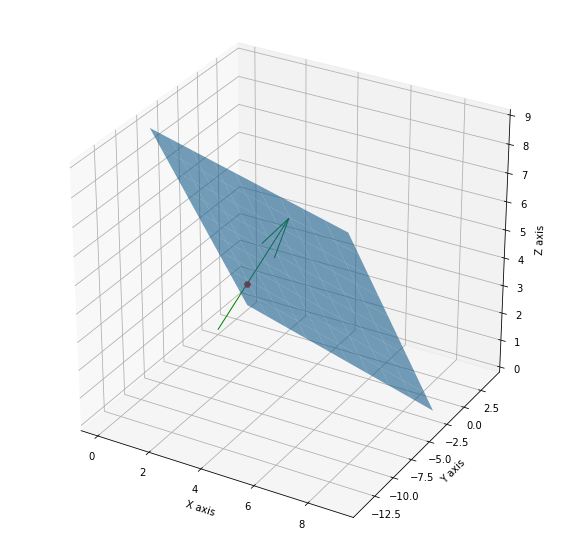
\includegraphics[width=\columnwidth]{plane1.png}
    \caption{Perpendicular drawn from origin to the plane $\myvec{2&3&4}\vec{x} = 12$}
    \label{myfig1}
\end{figure}
\renewcommand{\thefigure}{b}
\begin{figure}[h!]
    \centering
    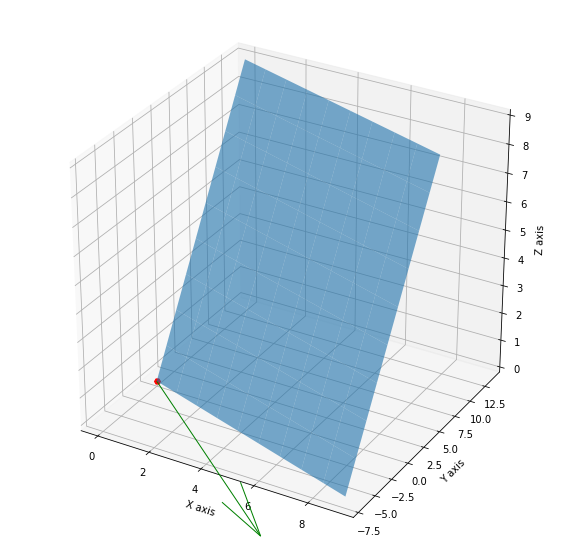
\includegraphics[width=\columnwidth]{plane2.png}
    \caption{Perpendicular drawn from origin to the plane $\myvec{3&4&-6}\vec{x} = 0$}
    \label{myfig2}
\end{figure}
\renewcommand{\thefigure}{c}
\begin{figure}[h!]
    \centering
    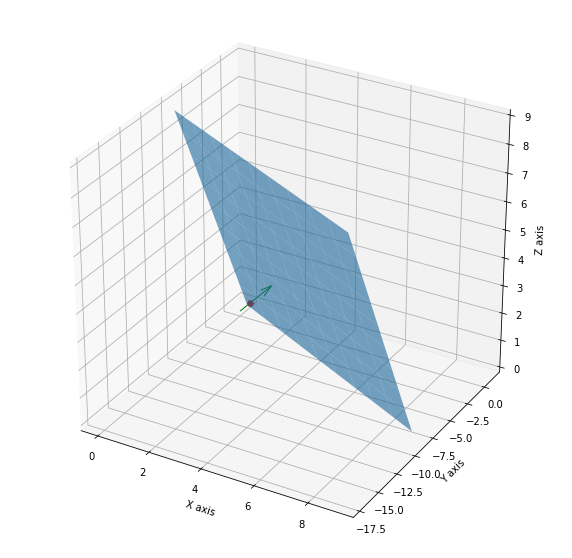
\includegraphics[width=\columnwidth]{plane3.png}
    \caption{Perpendicular drawn from origin to the plane $\myvec{1&1&1}\vec{x} = 1$}
    \label{myfig3}
\end{figure}
\renewcommand{\thefigure}{d}
\begin{figure}[h!]
    \centering
    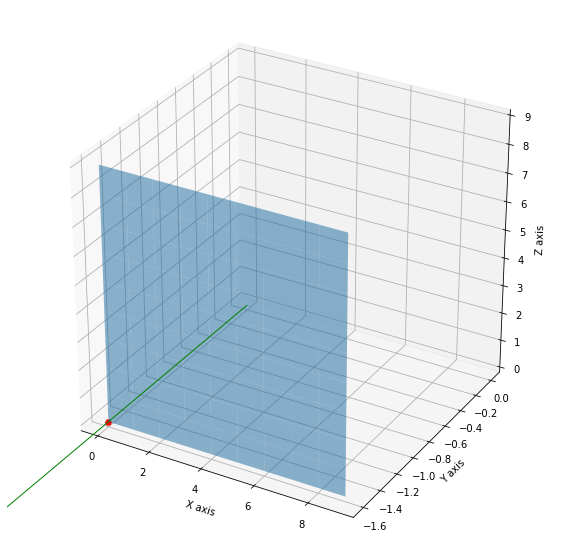
\includegraphics[width=\columnwidth]{plane4.png}
    \caption{Perpendicular drawn from origin to the plane $\myvec{0&5&0}\vec{x} = -8$}
    \label{myfig4}
\end{figure}
\end{document}